\documentclass[aspectratio=169]{beamer}

% ----------------------------------------------------------------------
% Codificación
% ----------------------------------------------------------------------
\usepackage[utf8]{inputenc}
\usepackage[T1]{fontenc}
\usepackage[main=spanish,provide=*]{babel}

% ----------------------------------------------------------------------
% Matemática y gráficos (mismos paquetes/librerías que el trabajo)
% ----------------------------------------------------------------------
\usepackage{amsmath,amssymb}
\usepackage{mathtools}
\usepackage{graphicx}
\usepackage{booktabs}
\usepackage{tabularx}
\usepackage{tikz}
\usepackage{tikz-3dplot}
\usepackage{pgfplots}
\pgfplotsset{compat=1.18}
\usetikzlibrary{calc,arrows.meta,positioning,decorations.markings,
                3d,backgrounds,fadings,shapes.geometric,patterns}
\usepackage{qrcode}

% ----------------------------------------------------------------------
% Tema base robusto (sin dependencias externas) + colores del trabajo
% ----------------------------------------------------------------------
\usetheme{Boadilla}
\usecolortheme{seahorse}
\setbeamertemplate{navigation symbols}{}
\setbeamercovered{transparent}

% ----------------------------------------------------------------------
% Paleta (copiada exacta del trabajo)
% ----------------------------------------------------------------------
\definecolor{navy}{HTML}{1B2A4A}
\definecolor{azul}{HTML}{2563A8}
\definecolor{rojo}{HTML}{C0392B}
\definecolor{verde}{HTML}{1F8A4C}
\definecolor{oro}{HTML}{B8860B}
\definecolor{gris}{HTML}{7A8699}
\definecolor{hielo}{HTML}{EEF3FA}

% Colores de Beamer con la paleta del trabajo
\setbeamercolor{frametitle}{bg=navy,fg=white}
\setbeamercolor{title}{fg=navy}
\setbeamercolor{structure}{fg=azul}
\setbeamercolor{alerted text}{fg=rojo}
\setbeamercolor{normal text}{fg=navy!92!black}
\setbeamercolor{itemize item}{fg=azul}
\setbeamercolor{itemize subitem}{fg=azul}
% Bloques: teorema en navy, definición en hielo
\setbeamercolor{block title}{bg=navy,fg=white}
\setbeamercolor{block body}{bg=hielo,fg=navy!92!black}
\setbeamercolor{block title alerted}{bg=rojo,fg=white}
\setbeamercolor{block body alerted}{bg=rojo!8,fg=navy!92!black}
\setbeamercolor{block title example}{bg=azul,fg=white}
\setbeamercolor{block body example}{bg=hielo,fg=navy!92!black}
\setbeamerfont{frametitle}{series=\bfseries}
\setbeamerfont{block title}{series=\bfseries}
\setbeamertemplate{blocks}[rounded][shadow=false]
\setbeamertemplate{itemize item}{\small\raise0.5pt\hbox{$\blacktriangleright$}}
\setbeamertemplate{itemize subitem}{\footnotesize\raise0.5pt\hbox{$\triangleright$}}

% ----------------------------------------------------------------------
% Notación (copiada del trabajo)
% ----------------------------------------------------------------------
\newcommand{\RP}{\mathbb{RP}}
\newcommand{\R}{\mathbb{R}}
\newcommand{\inc}[2]{\langle #1,\, #2\rangle}
\newcommand{\hp}[3]{[#1\,{:}\,#2\,{:}\,#3]}
\newcommand{\hpf}[4]{[#1\,{:}\,#2\,{:}\,#3\,{:}\,#4]}

% ----------------------------------------------------------------------
% Metadatos
% ----------------------------------------------------------------------
\title[Coordenadas homogéneas y dualidad]{Coordenadas homogéneas y dualidad}
\subtitle{Geometría proyectiva: del infinito a la visión por computadora}
\author{Carlos Nexans}
\institute[Geometría I]{\small Geometría I \;$\cdot$\; Licenciatura en Matemática}
\date{\today}

\begin{document}

% ======================================================================
% 1. PORTADA
% ======================================================================
{
\setbeamercolor{background canvas}{bg=navy}
\setbeamercolor{normal text}{fg=white}
\usebeamercolor[fg]{normal text}
\begin{frame}[plain]
  \vspace{0.6cm}
  \begin{center}
    {\color{oro!85!white}\footnotesize\bfseries
      GEOMETRÍA I \ \ {\color{azul!40!white}$\cdot$}\ \
      LICENCIATURA EN MATEMÁTICA}\\[1.0cm]
    {\color{white}\Huge\bfseries Coordenadas homogéneas}\\[0.25cm]
    {\color{white}\Huge\bfseries y dualidad}\\[0.5cm]
    {\color{oro!85!white}\large Geometría proyectiva: del infinito a la
      visión por computadora}\\[1.3cm]
    {\color{white}\large\bfseries Carlos Nexans}\\[0.2cm]
    {\color{gris!60!white}\small \today}
  \end{center}
\end{frame}
}

% ======================================================================
% 2. MOTIVACIÓN: DEL ESPACIO 3D AL PLANO (Y DE VUELTA)
% ======================================================================
\begin{frame}{Motivación: del espacio 3D al plano (y de vuelta)}
  \begin{columns}[T]
    \begin{column}{0.46\textwidth}
      \small
      \begin{itemize}
        \item La tecnología visual \textbf{traduce entre el espacio 3D y un
              plano 2D}.
        \item \textbf{3D $\rightarrow$ 2D:} una \alert{cámara} (o el ojo)
              recoge la luz de una escena y la proyecta sobre un plano: la
              foto, la pantalla.
        \item \textbf{2D $\rightarrow$ 3D:} con muchas mediciones, un
              \alert{LiDAR} reconstruye la nube de puntos que rodea a un
              auto autónomo.
      \end{itemize}
      \vspace{0.15cm}
      \begin{block}{El problema}
        Esa proyección \emph{no} es lineal en coordenadas usuales y manda
        los puntos lejanos \textbf{``al infinito''}. La \textbf{geometría
        proyectiva} es el lenguaje que la vuelve uniforme y lineal.
      \end{block}
    \end{column}
    \begin{column}{0.54\textwidth}
      \centering
      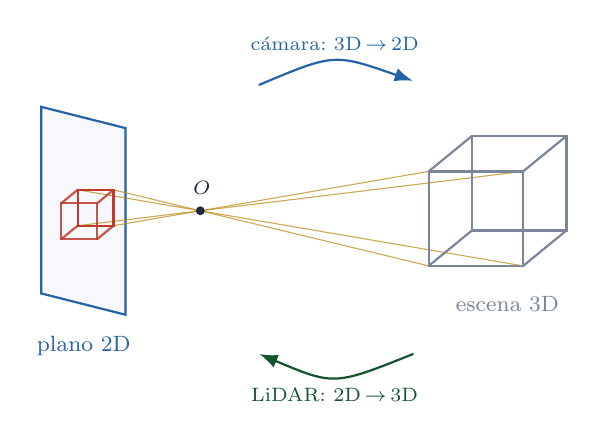
\begin{tikzpicture}[scale=1.0,>=Latex,line cap=round]
        % --- centro óptico O ---
        \coordinate (O) at (-1.3,0);
        % --- escena 3D: cubo grande ---
        \coordinate (F1) at (1.6,-0.7);  \coordinate (F2) at (2.8,-0.7);
        \coordinate (F3) at (2.8,0.5);   \coordinate (F4) at (1.6,0.5);
        \coordinate (K1) at (2.15,-0.25);\coordinate (K2) at (3.35,-0.25);
        \coordinate (K3) at (3.35,0.95); \coordinate (K4) at (2.15,0.95);
        % --- imagen del cubo en el plano (proyección invertida por O) ---
        \coordinate (f1) at (-2.402,0.266); \coordinate (f2) at (-2.858,0.266);
        \coordinate (f3) at (-2.858,-0.19); \coordinate (f4) at (-2.402,-0.19);
        \coordinate (k1) at (-2.611,0.095); \coordinate (k2) at (-3.067,0.095);
        \coordinate (k3) at (-3.067,-0.361);\coordinate (k4) at (-2.611,-0.361);
        % --- plano imagen (paralelogramo) ---
        \draw[azul,thick,fill=hielo,fill opacity=0.55]
              (-3.32,-1.05) -- (-2.25,-1.32) -- (-2.25,1.05) -- (-3.32,1.32) -- cycle;
        \node[azul,font=\footnotesize] at (-2.78,-1.72) {plano 2D};
        % --- rayos de proyección por O (frente del cubo) ---
        \foreach \B/\b in {F1/f1,F2/f2,F3/f3,F4/f4}{
          \draw[oro,thin,opacity=0.7] (\B) -- (\b);
        }
        % --- cubo imagen (rojo, invertido) ---
        \draw[rojo,thick] (f1)--(f2)--(f3)--(f4)--cycle;
        \draw[rojo,thick,opacity=0.85] (k1)--(k2)--(k3)--(k4)--cycle;
        \draw[rojo,thick,opacity=0.85] (f1)--(k1) (f2)--(k2) (f3)--(k3) (f4)--(k4);
        % --- cubo escena (gris) ---
        \draw[gris,thick] (F1)--(F2)--(F3)--(F4)--cycle;
        \draw[gris,thick] (K1)--(K2)--(K3)--(K4)--cycle;
        \draw[gris,thick] (F1)--(K1) (F2)--(K2) (F3)--(K3) (F4)--(K4);
        \node[gris,font=\footnotesize] at (2.6,-1.18) {escena 3D};
        % --- centro óptico ---
        \fill[navy] (O) circle (1.6pt);
        \node[navy,font=\scriptsize,above] at (-1.28,0.08) {$O$};
        % --- flechas de doble sentido ---
        \draw[->,azul,thick] (-0.55,1.6) .. controls (0.4,2.0) .. (1.4,1.65)
              node[midway,above,font=\scriptsize,azul]{cámara: $3$D\,$\to$\,$2$D};
        \draw[->,verde!60!black,thick] (1.4,-1.82) .. controls (0.4,-2.22) .. (-0.55,-1.82)
              node[midway,below,font=\scriptsize,verde!60!black]{LiDAR: $2$D\,$\to$\,$3$D};
      \end{tikzpicture}
    \end{column}
  \end{columns}
\end{frame}

% ======================================================================
% 2b. LA PROYECCIÓN EN CONCRETO: PUNTOS 3D -> PUNTOS 2D
% ======================================================================
\begin{frame}{Del punto 3D al punto 2D}
  \centering
  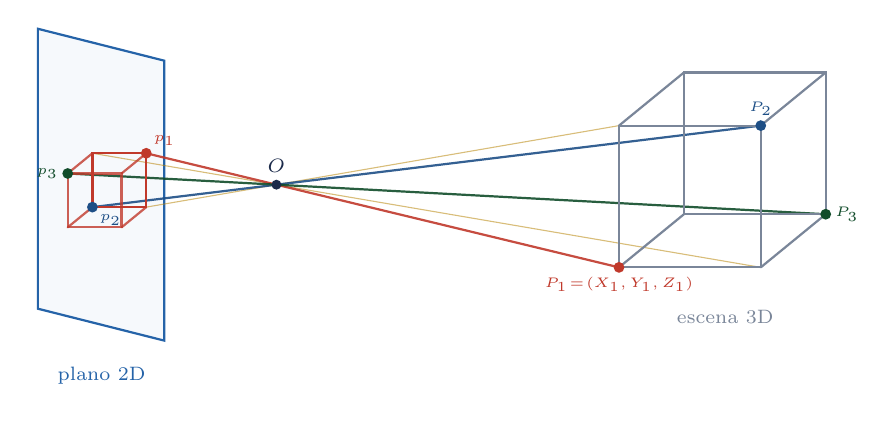
\begin{tikzpicture}[scale=1.5,>=Latex,line cap=round]
    \coordinate (O) at (-1.3,0);
    % --- escena 3D: cubo grande ---
    \coordinate (F1) at (1.6,-0.7);  \coordinate (F2) at (2.8,-0.7);
    \coordinate (F3) at (2.8,0.5);   \coordinate (F4) at (1.6,0.5);
    \coordinate (K1) at (2.15,-0.25);\coordinate (K2) at (3.35,-0.25);
    \coordinate (K3) at (3.35,0.95); \coordinate (K4) at (2.15,0.95);
    % --- imagen del cubo (proyección invertida por O) ---
    \coordinate (f1) at (-2.402,0.266); \coordinate (f2) at (-2.858,0.266);
    \coordinate (f3) at (-2.858,-0.19); \coordinate (f4) at (-2.402,-0.19);
    \coordinate (k1) at (-2.611,0.095); \coordinate (k2) at (-3.067,0.095);
    \coordinate (k3) at (-3.067,-0.361);\coordinate (k4) at (-2.611,-0.361);
    % --- plano imagen ---
    \draw[azul,thick,fill=hielo,fill opacity=0.5]
          (-3.32,-1.05) -- (-2.25,-1.32) -- (-2.25,1.05) -- (-3.32,1.32) -- cycle;
    \node[azul,font=\scriptsize] at (-2.78,-1.62) {plano $2$D};
    % --- rayos tenues (todos los vértices del frente) ---
    \foreach \B/\b in {F2/f2,F4/f4}{
      \draw[oro,thin,opacity=0.55] (\B) -- (\b);
    }
    % --- rayos destacados de los pares etiquetados ---
    \draw[rojo,thick,opacity=0.9] (F1) -- (f1);
    \draw[azul!80!black,thick,opacity=0.9] (F3) -- (f3);
    \draw[verde!55!black,thick,opacity=0.9] (K2) -- (k2);
    % --- cubo imagen (rojo) ---
    \draw[rojo,thick] (f1)--(f2)--(f3)--(f4)--cycle;
    \draw[rojo,thick,opacity=0.8] (k1)--(k2)--(k3)--(k4)--cycle;
    \draw[rojo,thick,opacity=0.8] (f1)--(k1) (f2)--(k2) (f3)--(k3) (f4)--(k4);
    % --- cubo escena (gris) ---
    \draw[gris,thick] (F1)--(F2)--(F3)--(F4)--cycle;
    \draw[gris,thick] (K1)--(K2)--(K3)--(K4)--cycle;
    \draw[gris,thick] (F1)--(K1) (F2)--(K2) (F3)--(K3) (F4)--(K4);
    \node[gris,font=\scriptsize] at (2.5,-1.12) {escena $3$D};
    % --- centro óptico ---
    \fill[navy] (O) circle (1.2pt);
    \node[navy,font=\scriptsize,above=1pt] at (O) {$O$};
    % --- pares destacados: puntos 3D y sus imágenes 2D ---
    \fill[rojo] (F1) circle (1.3pt);
    \node[rojo,font=\tiny,below=0pt] at (F1) {$P_1\!=\!(X_1,Y_1,Z_1)$};
    \fill[rojo] (f1) circle (1.3pt);
    \node[rojo,font=\tiny,above right=-1pt] at (f1) {$p_1$};
    \fill[azul!80!black] (F3) circle (1.3pt);
    \node[azul!80!black,font=\tiny,above=0pt] at (F3) {$P_2$};
    \fill[azul!80!black] (f3) circle (1.3pt);
    \node[azul!80!black,font=\tiny,below right=-1pt] at (f3) {$p_2$};
    \fill[verde!55!black] (K2) circle (1.3pt);
    \node[verde!55!black,font=\tiny,right=0pt] at (K2) {$P_3$};
    \fill[verde!55!black] (k2) circle (1.3pt);
    \node[verde!55!black,font=\tiny,left=0pt] at (k2) {$p_3$};
  \end{tikzpicture}

  \vspace{0.15cm}
  \begin{block}{De un mundo 3D a un punto 2D}
    \centering
    \large
    \textbf{\textcolor{navy}{$(X,\,Y,\,Z)$}}~$\longrightarrow$~\textbf{\textcolor{rojo}{$(u,\,v)$}}
    \hspace{1.4cm}\textcolor{gris}{\normalsize por ejemplo}\hspace{1.4cm}
    \textbf{\textcolor{navy}{$(2,\,1,\,5)$}}~$\longrightarrow$~\textbf{\textcolor{rojo}{$(410,\,205)$}}
  \end{block}
\end{frame}

% ======================================================================
% 3. CONTEXTO HISTÓRICO (timeline)
% ======================================================================
\begin{frame}{Contexto histórico}
  \centering
  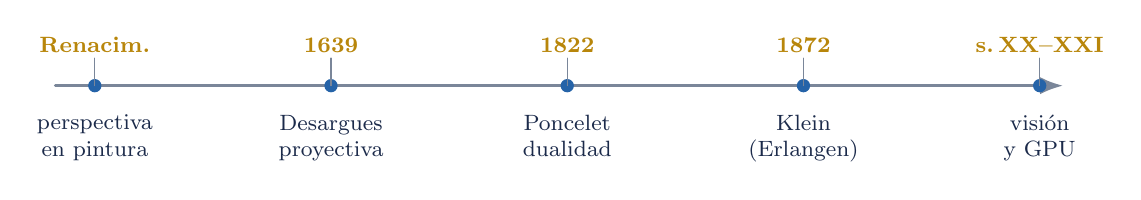
\begin{tikzpicture}[>=Latex,line cap=round,
      hito/.style={navy,font=\footnotesize,align=center}]
    \draw[gris,very thick,->] (-0.5,0) -- (12.3,0);
    \foreach \x/\ano/\txt in {
        0/Renacim./{perspectiva\\en pintura},
        3/1639/{Desargues\\proyectiva},
        6/1822/{Poncelet\\dualidad},
        9/1872/{Klein\\(Erlangen)},
        12/s.\,XX--XXI/{visión\\y GPU}}{
      \fill[azul] (\x,0) circle (2.4pt);
      \draw[gris] (\x,0) -- (\x,0.35);
      \node[oro,font=\footnotesize\bfseries,above=0.3cm] at (\x,0) {\ano};
      \node[hito,below=0.25cm] at (\x,0) {\txt};
    }
  \end{tikzpicture}
  \vspace{0.7cm}
  \begin{itemize}
    \item De una técnica de pintores a un lenguaje algebraico, y de ahí a
          los algoritmos que hoy mueven cámaras y GPUs.
  \end{itemize}
\end{frame}

% ======================================================================
% 4. EL MODELO: RECTAS POR EL ORIGEN
% ======================================================================
\begin{frame}{El modelo: rectas por el origen}
  \begin{columns}[T]
    \begin{column}{0.46\textwidth}
      \begin{itemize}
        \item Construimos $\RP^2$ a partir de $\R^3\setminus\{0\}$.
        \item Identificamos vectores proporcionales: $v\sim\lambda v$.
        \item \textbf{Un punto de $\RP^2$ es una recta por el origen} de
              $\R^3$.
      \end{itemize}
      \vspace{0.2cm}
      \begin{block}{Lectura geométrica}
        Las rectas que cortan $z=1$ dan puntos ordinarios; las contenidas en
        $z=0$ dan \alert{puntos al infinito}.
      \end{block}
    \end{column}
    \begin{column}{0.54\textwidth}
      \centering
      \tdplotsetmaincoords{70}{115}
      \resizebox{0.98\textwidth}{!}{%
      \begin{tikzpicture}[tdplot_main_coords,scale=2.0,
          line cap=round,line join=round,>=Latex]
        \fill[gris!35,opacity=0.55] (-1.4,-1.4,0) -- (1.4,-1.4,0) --
              (1.4,1.4,0) -- (-1.4,1.4,0) -- cycle;
        \node[gris] at (1.15,1.55,0) {\small $z=0$};
        \draw[->,gris!80!black] (0,0,0) -- (1.85,0,0) node[anchor=north east]{\small $x$};
        \draw[->,gris!80!black] (0,0,0) -- (0,1.85,0) node[anchor=west]{\small $y$};
        \draw[->,gris!80!black] (0,0,0) -- (0,0,1.75) node[anchor=south]{\small $z$};
        \draw[oro,very thick] (-1.3,-0.78,0) -- (1.3,0.78,0);
        \node[oro,anchor=north] at (1.2,0.74,0) {\small $\hp{x}{y}{0}$};
        \begin{scope}[opacity=0.85]
        \fill[azul!25] (-1.4,-1.4,1) -- (1.4,-1.4,1) --
              (1.4,1.4,1) -- (-1.4,1.4,1) -- cycle;
        \end{scope}
        \draw[azul!55,thin] (-1.4,-1.4,1) -- (1.4,-1.4,1) --
              (1.4,1.4,1) -- (-1.4,1.4,1) -- cycle;
        \node[azul] at (1.15,1.55,1) {\small $z=1$};
        \draw[rojo,thick] (-0.55,-0.35,-1) -- (0.66,0.42,1.2);
        \fill[rojo] (0.55,0.35,1) circle (1.4pt);
        \node[rojo,anchor=south east] at (0.5,0.32,1.08) {\small $P=\hp{x}{y}{z}$};
        \draw[verde,thick] (0.45,-0.7,-1) -- (-0.54,0.84,1.2);
        \fill[verde] (-0.45,0.7,1) circle (1.4pt);
        \fill[navy] (0,0,0) circle (1.4pt);
        \node[navy,anchor=north west] at (0.04,0,-0.04) {\small $O$};
      \end{tikzpicture}}
    \end{column}
  \end{columns}
\end{frame}

% ======================================================================
% 5. COORDENADAS HOMOGÉNEAS: DEFINICIÓN
% ======================================================================
\begin{frame}{Coordenadas homogéneas: definición}
  \begin{block}{Definición}
    Un punto de $\RP^2$ se escribe con \textbf{coordenadas homogéneas}
    \[
      P = \hp{x}{y}{z}, \qquad (x,y,z)\neq(0,0,0),
    \]
    con la convención de que las ternas proporcionales representan el mismo
    punto:
    \[
      (x,y,z)\ \sim\ (\lambda x,\lambda y,\lambda z),
      \qquad \lambda\neq 0.
    \]
  \end{block}
  \begin{itemize}
    \item Tres números para un objeto con \textbf{dos grados de libertad}:
          la escala global es irrelevante.
    \item De ahí «homogéneas»: si $f$ es homogéneo de grado $d$, entonces
          $f(\lambda x,\lambda y,\lambda z)=\lambda^d f(x,y,z)$, y
          \alert{anularse} queda bien definido sobre clases.
  \end{itemize}
\end{frame}

% ======================================================================
% 6. CARTA AFÍN Y PUNTOS AL INFINITO
% ======================================================================
\begin{frame}{Carta afín y puntos al infinito}
  \begin{columns}[T]
    \begin{column}{0.5\textwidth}
      \begin{itemize}
        \item Si $z\neq0$ normalizamos:
              \[
                \hp{x}{y}{z}\ \longleftrightarrow\
                \left(\tfrac{x}{z},\tfrac{y}{z}\right).
              \]
        \item Si $z=0$: $\hp{x}{y}{0}$ es el \alert{punto al infinito} en la
              dirección $y/x$.
        \item Las paralelas comparten ese punto; todos juntos forman
              $\ell_\infty$.
      \end{itemize}
      \vspace{0.1cm}
      \begin{block}{Descomposición}
        \[
          \RP^2 \;=\; \underbrace{\R^2}_{z\neq0}\ \sqcup\
          \underbrace{\ell_\infty}_{z=0}.
        \]
      \end{block}
    \end{column}
    \begin{column}{0.5\textwidth}
      \centering
      \resizebox{0.98\textwidth}{!}{%
      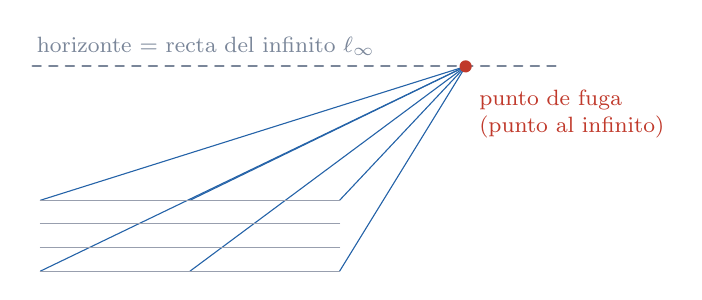
\begin{tikzpicture}[scale=1.0,>=Latex,line cap=round]
        \coordinate (V) at (5,1.6);
        \draw[gris,dashed,thick] (-0.5,1.6) -- (6.2,1.6);
        \node[gris,font=\footnotesize,above] at (1.7,1.62)
              {horizonte $=$ recta del infinito $\ell_\infty$};
        \foreach \x in {-0.4,1.5,3.4}{
          \draw[azul] (\x,-0.1) -- (V);
          \draw[azul] (\x,-1.0) -- (V);
        }
        \foreach \y in {-0.1,-0.4,-0.7,-1.0}{
          \draw[navy!45,thin] (-0.4,\y) -- (3.4,\y);
        }
        \fill[rojo] (V) circle (2.2pt);
        \node[rojo,below right,align=left,font=\footnotesize] at ($(V)+(0.05,-0.18)$)
              {punto de fuga\\(punto al infinito)};
      \end{tikzpicture}}
    \end{column}
  \end{columns}
\end{frame}

% ======================================================================
% 7. RECTAS E INCIDENCIA
% ======================================================================
\begin{frame}{Rectas e incidencia}
  \begin{itemize}
    \item Una recta se describe \emph{igual que un punto}: una terna
          $\ell=\hp{a}{b}{c}$ salvo escala.
  \end{itemize}
  \vspace{0.2cm}
  \begin{block}{Condición de incidencia}
    \centering\large
    $\displaystyle P\in\ell \iff \inc{P}{\ell}=ax+by+cz=0.$
  \end{block}
  \vspace{0.2cm}
  \begin{itemize}
    \item El producto escalar $\inc{P}{\ell}=ax+by+cz$ es
          \alert{perfectamente simétrico}: intercambiar $P$ y $\ell$ no lo
          altera.
    \item Esa simetría \emph{puramente algebraica} es la \textbf{semilla de
          todo el principio de dualidad}.
  \end{itemize}
\end{frame}

% ======================================================================
% 8. UNIR Y CORTAR: PRODUCTO VECTORIAL
% ======================================================================
\begin{frame}{Unir y cortar: el producto vectorial}
  \begin{columns}[T]
    \begin{column}{0.46\textwidth}
      \[
        \underbrace{\ell = P_1\times P_2}_{\text{une dos puntos}}
        \quad
        \underbrace{P = \ell_1\times \ell_2}_{\text{corta dos rectas}}
      \]
      \begin{itemize}
        \item $P_1\times P_2$ es ortogonal a $P_1$ y $P_2$: ambos en $\ell$.
        \item Una sola operación, dos problemas (perfectamente duales).
      \end{itemize}
      \pause
      \begin{block}{Sin excepciones}
        Dos rectas distintas siempre se cortan: si son paralelas, el
        producto entrega un \alert{punto al infinito}.
      \end{block}
    \end{column}
    \begin{column}{0.54\textwidth}
      \centering
      \resizebox{0.98\textwidth}{!}{%
      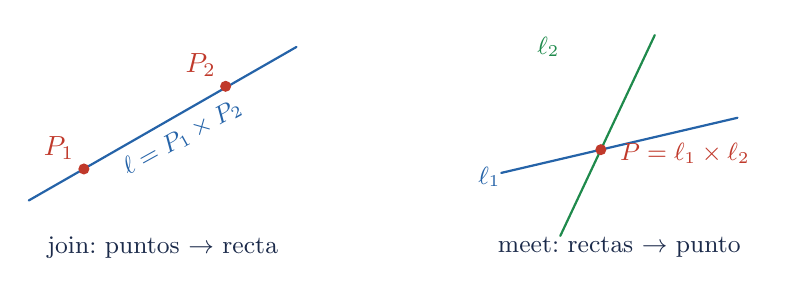
\begin{tikzpicture}[scale=1.0,>=Latex,line cap=round]
        \begin{scope}
          \draw[azul,thick] (-0.4,-0.1) -- (3.0,1.85);
          \fill[rojo] (0.3,0.3) circle (2pt) node[above left,rojo]{$P_1$};
          \fill[rojo] (2.1,1.35) circle (2pt) node[above left,rojo]{$P_2$};
          \node[azul,rotate=29] at (1.55,0.7) {\small $\ell=P_1\times P_2$};
          \node[navy] at (1.3,-0.7) {\small join: puntos $\to$ recta};
        \end{scope}
        \begin{scope}[xshift=6.0cm]
          \coordinate (L1a) at (-0.4,0.25);
          \coordinate (L1b) at (2.6,0.95);
          \coordinate (L2a) at (0.35,-0.55);
          \coordinate (L2b) at (1.55,2.0);
          \draw[azul,thick]  (L1a) -- (L1b);
          \draw[verde,thick] (L2a) -- (L2b);
          \coordinate (P) at (intersection of L1a--L1b and L2a--L2b);
          \fill[rojo] (P) circle (2pt);
          \node[rojo,right] at ($(P)+(0.12,-0.05)$) {\small $P=\ell_1\times\ell_2$};
          \node[azul]  at (-0.55,0.2) {\small $\ell_1$};
          \node[verde] at (0.2,1.85)  {\small $\ell_2$};
          \node[navy]  at (1.1,-0.7)  {\small meet: rectas $\to$ punto};
        \end{scope}
      \end{tikzpicture}}
    \end{column}
  \end{columns}
\end{frame}

% ======================================================================
% 9. (RECORTABLE) RP^2 NO ES ESPACIO VECTORIAL
% ======================================================================
\begin{frame}{$\RP^2$ no es un espacio vectorial}
  \begin{itemize}
    \item La suma de $\R^3$ \alert{no desciende} al cociente: $v\sim\lambda v$
          pero $v+w\not\sim\lambda v+w$.
    \item Lo que sí baja son los \textbf{subespacios}, perdiendo una
          dimensión: recta de $\R^3$ $\to$ punto; plano $\to$ recta.
  \end{itemize}
  \vspace{0.2cm}
  \begin{block}{Consecuencia (fórmula de dimensión)}
    Dos planos distintos de $\R^3$ se cortan en una recta
    ($2+2-3=1$); proyectivamente, \textbf{dos rectas de $\RP^2$ siempre se
    cortan en un punto}. Sin paralelas, sin excepciones.
  \end{block}
\end{frame}

% ======================================================================
% 9a. EL ESPACIO PROYECTIVO P(E) EN GENERAL
% ======================================================================
\begin{frame}{El espacio proyectivo $\mathbb P(E)$ en general}
  \begin{block}{Definición}
    Dado un espacio vectorial $E$, el \textbf{espacio proyectivo}
    $\mathbb P(E)$ es el conjunto de sus \textbf{rectas por el origen}
    (los subespacios de dimensión $1$). Equivalentemente,
    \[
      \mathbb P(E) \;=\; (E\setminus\{\mathbf 0\})\,/\!\sim,
      \qquad v \sim \lambda v \ \ (\lambda\neq 0).
    \]
  \end{block}
  \begin{columns}[T]
    \begin{column}{0.5\textwidth}
      \begin{itemize}
        \item Cocientar por la escala \alert{quita un grado de libertad}:
              \[ \dim \mathbb P(E) = \dim E - 1. \]
        \item $\RP^n := \mathbb P(\R^{n+1})$; \;
              en particular $\RP^2=\mathbb P(\R^3)$ —el caso que venimos
              usando—.
      \end{itemize}
    \end{column}
    \begin{column}{0.5\textwidth}
      \begin{block}{Subespacios proyectivos}
        Un subespacio $L=\mathbb P(V)$ proviene de un subespacio vectorial
        $V\subseteq E$, con
        \[ \dim L = \dim V - 1. \]
        {\footnotesize
        recta de $\R^3$ ($\dim 1$) $\to$ punto;\\
        plano de $\R^3$ ($\dim 2$) $\to$ recta.}
      \end{block}
    \end{column}
  \end{columns}
\end{frame}

% ======================================================================
% 9b. LA FÓRMULA DE DIMENSIÓN
% ======================================================================
\begin{frame}{La fórmula de dimensión}
  \begin{itemize}
    \item Recordemos: $\dim\mathbb P(V)=\dim V-1$, así que punto $=0$, \;
          recta $=1$, \; $\RP^2=2$; \; y por convención $\dim\varnothing=-1$.
  \end{itemize}
  \vspace{0.1cm}
  \begin{block}{Fórmula de dimensión (Santaló)}
    Para subespacios $L_r,\,M_p \subseteq \RP^n$ de dimensiones $r$ y $p$,
    \[
      \dim L_r + \dim M_p \;=\; \dim(L_r + M_p) \,+\, \dim(L_r \cap M_p),
    \]
    con la convención $\dim\varnothing=-1$ (para que valga incluso cuando
    no se cortan).
  \end{block}
  \vspace{0.1cm}
  \begin{columns}[T]
    \begin{column}{0.48\textwidth}
      \begin{block}{Consecuencia}
        Si $\,r+p \ge n$, los subespacios \alert{siempre se cortan}.
      \end{block}
    \end{column}
    \begin{column}{0.48\textwidth}
      \begin{block}{Caso $r=p=1$, $n=2$}
        Dos rectas de $\RP^2$ ($1+1\ge 2$): \textbf{un único punto común}.
      \end{block}
    \end{column}
  \end{columns}
\end{frame}

% ======================================================================
% 10. EL PRINCIPIO DE DUALIDAD
% ======================================================================
\begin{frame}{El principio de dualidad}
  \begin{block}{Principio de dualidad en el plano}
    Todo enunciado válido en $\RP^2$ sigue siendo válido al intercambiar
    \textbf{punto $\leftrightarrow$ recta} (y «pasar por» $\leftrightarrow$
    «estar sobre»). Cada teorema viene con su \alert{dual gratis}.
  \end{block}
  \vspace{0.2cm}
  \centering
  \begin{tabular}{r c l}
    \toprule
    \textbf{primal} & $\xleftrightarrow{\ \delta\ }$ & \textbf{dual}\\
    \midrule
    punto $P$ & & recta $\ell$\\
    \onslide<2->{recta que une 2 puntos} & \onslide<2->{} & \onslide<2->{punto donde se cortan 2 rectas}\\
    \onslide<3->{puntos colineales} & \onslide<3->{} & \onslide<3->{rectas concurrentes}\\
    \onslide<4->{$\inc{P}{\ell}=0$} & \onslide<4->{} & \onslide<4->{$\inc{\ell}{P}=0$}\\
    \bottomrule
  \end{tabular}
\end{frame}

% ======================================================================
% 10b. DUALIDAD EN DIMENSIÓN n: PUNTO <-> HIPERPLANO
% ======================================================================
\begin{frame}{Dualidad en general: punto $\leftrightarrow$ hiperplano}
  \begin{itemize}
    \item El par punto $\leftrightarrow$ recta es \emph{propio de} $\RP^2$.
          La regla general intercambia las dimensiones:
  \end{itemize}
  \[
    L_r \;\longleftrightarrow\; L_{\,n-r-1}.
  \]
  \begin{itemize}
    \item Un \textbf{punto} ($r=0$) se dualiza con $L_{n-1}$: un
          \textbf{hiperplano} (codimensión $1$).
  \end{itemize}
  \vspace{0.1cm}
  \begin{columns}[T]
    \begin{column}{0.48\textwidth}
      \begin{block}{En $\RP^2$ ($n=2$)}
        Un hiperplano \emph{es} una recta ($n-1=1$): la dualidad colapsa
        al par \textbf{punto $\leftrightarrow$ recta}.
      \end{block}
    \end{column}
    \begin{column}{0.48\textwidth}
      \begin{block}{En $\RP^3$ ($n=3$)}
        Punto $\leftrightarrow$ plano; y una \textbf{recta} ($r=1$) se
        dualiza con $L_{1}$: ¡las rectas son \alert{autoduales}!
      \end{block}
    \end{column}
  \end{columns}
\end{frame}

% ======================================================================
% 11. COLINEALIDAD Y CONCURRENCIA
% ======================================================================
\begin{frame}{Colinealidad y concurrencia}
  \begin{columns}[T]
    \begin{column}{0.42\textwidth}
      \[
        \det[P_1\,P_2\,P_3]=0
        \ \xleftrightarrow{\ \delta\ }\
        \det[\ell_1\,\ell_2\,\ell_3]=0
      \]
      \begin{itemize}
        \item Tres puntos colineales $\iff$ determinante nulo.
        \item Su dual: tres rectas concurrentes.
        \item Triple producto:
              \[
                \det = (P_1\times P_2)\cdot P_3 = \inc{P_3}{\ell}.
              \]
      \end{itemize}
    \end{column}
    \begin{column}{0.58\textwidth}
      \centering
      \resizebox{0.98\textwidth}{!}{%
      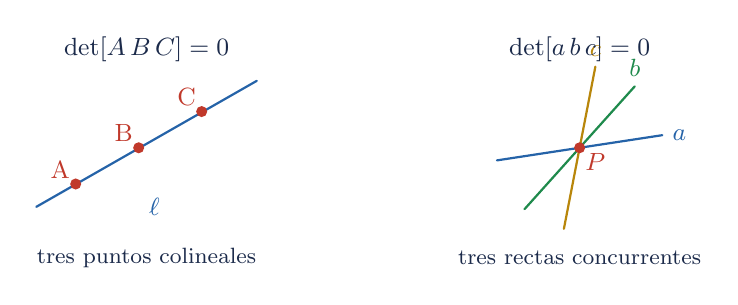
\begin{tikzpicture}[scale=1.0,>=Latex,line cap=round]
        \begin{scope}
          \draw[azul,thick] (-0.3,-0.05) -- (2.5,1.55);
          \foreach \x/\y/\l in {0.2/0.24/A, 1.0/0.7/B, 1.8/1.16/C}{
            \fill[rojo] (\x,\y) circle (2pt);
            \node[rojo,above left=-2pt] at (\x,\y) {\small \l};
          }
          \node[azul] at (1.2,-0.05) {\small $\ell$};
          \node[navy] at (1.1,1.95) {\small $\det[A\,B\,C]=0$};
          \node[navy,font=\footnotesize] at (1.1,-0.7) {tres puntos colineales};
        \end{scope}
        \begin{scope}[xshift=5.6cm]
          \coordinate (P) at (1.0,0.7);
          \draw[azul,thick]  ($(P)+(-1.05,-0.16)$) -- ($(P)+(1.05,0.16)$) node[right]{\small $a$};
          \draw[verde,thick] ($(P)+(-0.7,-0.78)$)  -- ($(P)+(0.7,0.78)$)  node[above]{\small $b$};
          \draw[oro,thick]   ($(P)+(-0.2,-1.03)$)  -- ($(P)+(0.2,1.03)$)  node[above]{\small $c$};
          \fill[rojo] (P) circle (2pt);
          \node[rojo,below right=-2pt] at (P) {\small $P$};
          \node[navy] at (1.0,1.95) {\small $\det[a\,b\,c]=0$};
          \node[navy,font=\footnotesize] at (1.0,-0.7) {tres rectas concurrentes};
        \end{scope}
      \end{tikzpicture}}
    \end{column}
  \end{columns}
\end{frame}

% ======================================================================
% 12. (RECORTABLE) DUALIDAD COMO METATEOREMA
% ======================================================================
\begin{frame}{Dualidad como metateorema}
  La dualidad no es un teorema más: \textbf{habla sobre los teoremas} y
  «regala el doble». Aparece siempre que los axiomas son simétricos.
  \vspace{0.3cm}
  \begin{columns}[T]
    \begin{column}{0.32\textwidth}
      \begin{block}{Geometría}
        punto $\leftrightarrow$ recta\\[2pt]
        Pascal $\leftrightarrow$ Brianchon
      \end{block}
    \end{column}
    \begin{column}{0.34\textwidth}
      \begin{block}{Lógica}
        $\neg(p\wedge q)\equiv\neg p\vee\neg q$\\[2pt]
        $\neg\forall \equiv \exists\,\neg$
      \end{block}
    \end{column}
    \begin{column}{0.32\textwidth}
      \begin{block}{Conjuntos}
        $\overline{A\cup B}=\bar A\cap\bar B$\\[2pt]
        $\cup \leftrightarrow \cap$
      \end{block}
    \end{column}
  \end{columns}
  \vspace{0.3cm}
  \begin{itemize}
    \item Axiomas simétricos bajo el intercambio $\Rightarrow$ la simetría se
          \alert{hereda} a todo teorema demostrado a partir de ellos.
  \end{itemize}
\end{frame}

% ======================================================================
% 13. HOMOGRAFÍAS Y PGL_3(R)
% ======================================================================
\begin{frame}{Homografías y $\mathrm{PGL}_3(\R)$}
  \begin{block}{Definición}
    \textbf{En palabras:} las homografías son el \textbf{grupo de
    transformaciones del plano proyectivo} $\RP^2$ —las biyecciones que
    preservan su estructura: llevan rectas a rectas y respetan la
    incidencia—.
    \smallskip

    \textbf{Formalmente:} $\lambda x' = Hx$ con $H\in \mathrm{GL}_3(\R)$,
    identificando $H\sim\mu H$. El grupo es
    $\mathrm{PGL}_3(\R)=\mathrm{GL}_3(\R)/\R^\times$, de
    \textbf{dimensión $8$}.
  \end{block}
  \begin{columns}[T]
    \begin{column}{0.5\textwidth}
      \begin{itemize}
        \item $9$ entradas $-1$ por escala $=$ \textbf{8 grados de libertad}.
        \item $4$ pares de puntos en posición general \alert{fijan} $H$.
      \end{itemize}
    \end{column}
    \begin{column}{0.5\textwidth}
      \begin{itemize}
        \item \textbf{Preservan:} incidencia, colinealidad, razón doble.
        \item \textbf{No preservan:} distancias, ángulos, paralelismo.
      \end{itemize}
    \end{column}
  \end{columns}
\end{frame}

% ======================================================================
% 14. HOMOGRAFÍA EN ACCIÓN: MOVER EL INFINITO
% ======================================================================
\begin{frame}{Homografía en acción: mover el infinito}
  \begin{columns}[T]
    \begin{column}{0.5\textwidth}
      \[
        H=\begin{pmatrix} 1&0&0\\ 0&1&0\\ 1&0&1 \end{pmatrix}
      \]
      \begin{itemize}
        \item Tomamos el punto al infinito $[1:0:0]$:
              \[
                H\begin{pmatrix}1\\0\\0\end{pmatrix}
                =\begin{pmatrix}1\\0\\1\end{pmatrix}
                = [1:0:1] \to (1,0).
              \]
        \item ¡Un punto al infinito se volvió \alert{finito}!
      \end{itemize}
    \end{column}
    \begin{column}{0.5\textwidth}
      \begin{block}{Por qué importa}
        \textbf{Ninguna transformación afín} puede hacer esto: fijan
        $\ell_\infty$. Mover el infinito a una posición finita (o al revés)
        es exactamente lo que hace la \alert{rectificación de documentos}
        —enderezar una foto tomada en ángulo—, una aplicación que veremos
        más adelante.
      \end{block}
    \end{column}
  \end{columns}
\end{frame}

% ======================================================================
% 15. TEOREMA DE DESARGUES (AUTODUAL)
% ======================================================================
\begin{frame}{Teorema de Desargues (autodual)}
  \begin{columns}[T]
    \begin{column}{0.46\textwidth}
      \begin{block}{Desargues}
        Si dos triángulos están en \textbf{perspectiva desde un punto} $O$
        (rectas $AA',BB',CC'$ concurrentes), entonces los lados
        correspondientes se cortan en tres puntos \alert{colineales}
        $X,Y,Z$.
      \end{block}
      \begin{itemize}
        \item \textbf{Autodual:} $\delta$ intercambia hipótesis y conclusión;
              el dual \emph{coincide} con el recíproco.
      \end{itemize}
    \end{column}
    \begin{column}{0.54\textwidth}
      \centering
      \resizebox{0.62\textwidth}{!}{%
      \begin{tikzpicture}[scale=0.62,>=Latex,line cap=round]
        \coordinate (O)  at (0,0);
        \coordinate (A)  at (1.2,2.6);
        \coordinate (B)  at (2.8,1.0);
        \coordinate (C)  at (1.0,0.5);
        \coordinate (Ap) at ($(O)!1.75!(A)$);
        \coordinate (Bp) at ($(O)!1.55!(B)$);
        \coordinate (Cp) at ($(O)!2.3!(C)$);
        \foreach \p in {Ap,Bp,Cp}{ \draw[gris,dashed] (O) -- (\p); }
        \draw[azul,thick] (A)--(B)--(C)--cycle;
        \draw[rojo,thick] (Ap)--(Bp)--(Cp)--cycle;
        \coordinate (X) at (intersection of A--B and Ap--Bp);
        \coordinate (Y) at (intersection of B--C and Bp--Cp);
        \coordinate (Z) at (intersection of C--A and Cp--Ap);
        \draw[oro,thick] (X) -- (Z);
        \foreach \p in {X,Y,Z}{ \fill[oro] (\p) circle (1.8pt); }
        \node[oro] at ($(X)+(0.0,0.25)$) {\small $X$};
        \node[oro] at ($(Y)+(0.25,0.05)$) {\small $Y$};
        \node[oro] at ($(Z)+(-0.2,0.18)$) {\small $Z$};
        \foreach \p/\l/\pos in {O/O/below left, A/A/above left, B/B/below,
              C/C/below left, Ap/A'/above, Bp/B'/right, Cp/C'/left}{
          \fill[navy] (\p) circle (1.6pt);
          \node[navy,\pos=1pt,font=\footnotesize] at (\p) {$\l$};
        }
      \end{tikzpicture}}
    \end{column}
  \end{columns}
\end{frame}

% ======================================================================
% 16. PASCAL <-> BRIANCHON
% ======================================================================
\begin{frame}{Pascal $\leftrightarrow$ Brianchon}
  \begin{columns}[T]
    \begin{column}{0.5\textwidth}
      \begin{block}{Pascal (1640)}
        Hexágono \textbf{inscrito} en una cónica $\Rightarrow$ los tres pares
        de lados opuestos se cortan en \alert{3 puntos colineales}.
      \end{block}
    \end{column}
    \begin{column}{0.5\textwidth}
      \begin{block}{Brianchon (1806) — dual}
        Hexágono \textbf{circunscrito} a una cónica $\Rightarrow$ las tres
        diagonales son \alert{3 rectas concurrentes}.
      \end{block}
    \end{column}
  \end{columns}
  \vspace{0.4cm}
  \begin{itemize}
    \item Dos teoremas separados por casi dos siglos: la dualidad los muestra
          como \textbf{uno solo}.
    \item Cuidado: \emph{dual $\neq$ recíproco}; aquí cada uno se obtiene
          gratis del otro intercambiando punto $\leftrightarrow$ recta.
  \end{itemize}
\end{frame}

% ======================================================================
% 17. (RECORTABLE) JERARQUÍA DE GEOMETRÍAS (ERLANGEN)
% ======================================================================
\begin{frame}{Jerarquía de geometrías (programa de Erlangen)}
  \begin{block}{Idea de Klein}
    Una geometría $=$ el estudio de los \textbf{invariantes de un grupo} de
    transformaciones. A más grupo, menos invariantes.
  \end{block}
  \vspace{0.2cm}
  \centering
  \begin{tabular}{l l l}
    \toprule
    \textbf{Geometría} & \textbf{Grupo} & \textbf{Invariantes}\\
    \midrule
    Euclidiana & isometrías & distancias, ángulos\\
    Similar    & semejanzas & ángulos, razones\\
    Afín       & afinidades & paralelismo, razón en una recta\\
    \textbf{Proyectiva} & \textbf{homografías} & incidencia, razón doble\\
    \bottomrule
  \end{tabular}
  \vspace{0.3cm}
  \begin{itemize}
    \item Euclidiana $\subset$ Similar $\subset$ Afín $\subset$
          \alert{Proyectiva}: en el fondo, la más simétrica. Las otras se
          obtienen \emph{fijando} estructura ($\ell_\infty$, una cónica\ldots).
  \end{itemize}
\end{frame}

% ======================================================================
% 18. APLICACIÓN: CÁMARA ESTENOPEICA
% ======================================================================
\begin{frame}{Aplicación: la cámara estenopeica}
  \begin{columns}[T]
    \begin{column}{0.4\textwidth}
      \[
        \lambda\!\begin{pmatrix}u\\v\\1\end{pmatrix}
        = K\,[R\mid t]\!
        \begin{pmatrix}X\\Y\\Z\\1\end{pmatrix}
      \]
      \begin{itemize}
        \item Mundo en $\RP^3$ (4 componentes).
        \item Subir de dimensión vuelve el modelo \alert{lineal}.
        \item $\div w'$ $=$ carta afín $\to$ píxeles.
        \item $K$: intrínsecos; $[R\mid t]$: extrínsecos (pose).
      \end{itemize}
    \end{column}
    \begin{column}{0.6\textwidth}
      \centering
      \resizebox{0.98\textwidth}{!}{%
      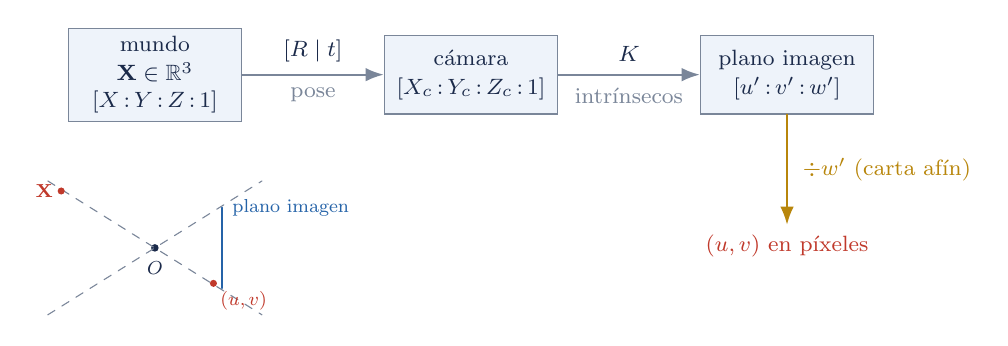
\begin{tikzpicture}[
          >=Latex,line cap=round,
          box/.style={navy,align=center,font=\footnotesize,
                      inner sep=3pt,minimum height=10mm,minimum width=22mm,
                      draw=gris,fill=hielo},
          arr/.style={->,gris,thick},
          arrlab/.style={navy,font=\footnotesize},
          arrlow/.style={gris,font=\footnotesize}]
        \node[box] (mundo)
          {mundo\\[1pt]$\mathbf{X}\in\R^3$\\\footnotesize$\hpf{X}{Y}{Z}{1}$};
        \node[box,right=18mm of mundo] (cam)
          {cámara\\[1pt]$\hpf{X_c}{Y_c}{Z_c}{1}$};
        \node[box,right=18mm of cam] (img)
          {plano imagen\\[1pt]$\hp{u'}{v'}{w'}$};
        \draw[arr] (mundo) -- (cam)
              node[midway,above=1pt,arrlab]{$[R\mid t]$}
              node[midway,below=1pt,arrlow]{pose};
        \draw[arr] (cam) -- (img)
              node[midway,above=1pt,arrlab]{$K$}
              node[midway,below=1pt,arrlow]{intrínsecos};
        \node[rojo,font=\footnotesize,below=14mm of img] (px) {$(u,v)$ en píxeles};
        \draw[->,oro,thick] (img) -- (px)
              node[midway,right=2pt,oro,font=\footnotesize]{$\div w'$ (carta afín)};
        \begin{scope}[xshift=0mm,yshift=-22mm,scale=0.85,every node/.style={transform shape}]
          \fill[navy] (0,0) circle (1.6pt);
          \node[navy,font=\footnotesize,below] at (0,-0.08) {$O$};
          \draw[gris,dashed] (-1.6,1.0) -- (0,0) -- (1.6,-1.0);
          \draw[gris,dashed] (-1.6,-1.0) -- (0,0) -- (1.6,1.0);
          \draw[azul,thick] (1.0,-0.6) -- (1.0,0.6);
          \node[azul,font=\footnotesize,right=1pt] at (1.0,0.6) {plano imagen};
          \fill[rojo] (-1.4,0.85) circle (1.5pt);
          \node[rojo,font=\footnotesize,left] at (-1.4,0.85) {$\mathbf{X}$};
          \fill[rojo] (0.875,-0.53) circle (1.5pt);
          \node[rojo,font=\footnotesize,below right=-1pt] at (0.88,-0.55) {$(u,v)$};
        \end{scope}
      \end{tikzpicture}}
    \end{column}
  \end{columns}
\end{frame}

% ======================================================================
% 19. EJEMPLO NUMÉRICO: PEATÓN A 10 m
% ======================================================================
\begin{frame}{Ejemplo numérico: peatón a 10 m}
  \begin{columns}[T]
    \begin{column}{0.32\textwidth}
      {\footnotesize
      $K$: $f=1000$, centro $(640,360)$;\\
      $R=I$, $t=(-1,0,0)$;\\
      mundo $X=(0,0,10)$.}
    \end{column}
    \begin{column}{0.42\textwidth}
      \onslide<2->{%
      \begin{block}{}
        \vspace{-2pt}{\footnotesize
        $(0,0,10)\!+\!(-1,0,0)\!\to\!(-1,0,10)$\\[2pt]
        $K(-1,0,10)\to(5400,3600,10)$\\[2pt]
        $\div 10 \to (540,360)$.}\vspace{-2pt}
      \end{block}}
    \end{column}
    \begin{column}{0.26\textwidth}
      \onslide<3->{%
      {\footnotesize $\tan\theta=\tfrac1{10}\Rightarrow$ \alert{100 px} del
       centro.}}
    \end{column}
  \end{columns}
  \vspace{0.1cm}
  \begin{center}
      \resizebox{!}{5.0cm}{%
      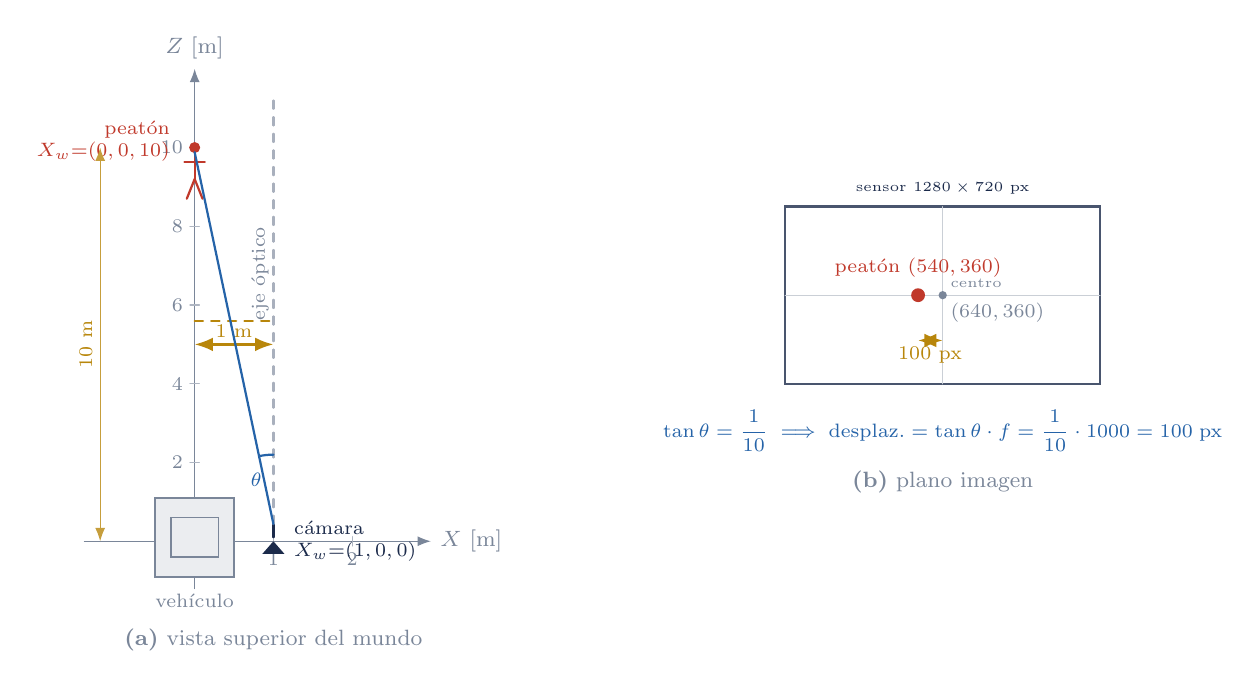
\begin{tikzpicture}[>=Latex,line cap=round]
        \begin{scope}
          \draw[->,gris] (-1.4,0) -- (3.0,0) node[right,gris,font=\footnotesize]{$X$ [m]};
          \draw[->,gris] (0,-0.6) -- (0,6.0) node[above,gris,font=\footnotesize]{$Z$ [m]};
          \node[gris,font=\scriptsize,below left=-2pt] at (0,0) {$O_w$};
          \foreach \x in {1,2}{
            \draw[gris!60] (\x,-0.06) -- (\x,0.06);
            \node[gris,font=\scriptsize,below=-1pt] at (\x,-0.06) {\x};
          }
          \foreach \z in {1,2,3,4,5}{
            \draw[gris!60] (-0.06,\z) -- (0.06,\z);
            \pgfmathtruncatemacro{\zm}{\z*2}
            \node[gris,font=\scriptsize,left=-1pt] at (-0.06,\z) {\zm};
          }
          \fill[gris!15]   (-0.5,-0.45) rectangle (0.5,0.55);
          \draw[gris,thick] (-0.5,-0.45) rectangle (0.5,0.55);
          \draw[gris,thin]  (-0.3,-0.2)  rectangle (0.3,0.30);
          \node[gris,font=\scriptsize] at (0,-0.75) {vehículo};
          \fill[navy] (1,0.0) -- (0.86,-0.16) -- (1.14,-0.16) -- cycle;
          \draw[navy,thick] (1,0.05) -- (1,0.22);
          \node[navy,font=\scriptsize,right=4pt,align=left]
                at (1.0,0.0) {cámara\\$X_w{=}(1,0,0)$};
          \draw[gris!65,dashed,thick] (1,0.22) -- (1,5.7);
          \node[gris,font=\scriptsize,rotate=90] at (0.83,3.4) {eje óptico};
          \fill[rojo] (0,5) circle (2pt);
          \draw[rojo,thick] (0,4.94) -- (0,4.6);
          \draw[rojo,thick] (-0.13,4.82) -- (0.13,4.82);
          \draw[rojo,thick] (0,4.6) -- (-0.1,4.35);
          \draw[rojo,thick] (0,4.6) -- (0.1,4.35);
          \node[rojo,font=\scriptsize,left=4pt,align=right]
                at (-0.05,5.08) {peatón\\$X_w{=}(0,0,10)$};
          \draw[oro,thick,dashed] (0,2.8) -- (1,2.8);
          \draw[oro,thick,<->]    (0,2.5) -- (1,2.5);
          \node[oro,font=\scriptsize,above=-1pt] at (0.5,2.5) {$1$ m};
          \draw[oro!80,thin,<->] (-1.2,0.0) -- (-1.2,5.0);
          \node[oro,font=\scriptsize,rotate=90] at (-1.38,2.5) {$10$ m};
          \draw[azul,thick] (1,0.22) -- (0,4.94);
          \draw[azul,thick] (1,1.10) arc[start angle=90,end angle=101.6,radius=0.88];
          \node[azul] at (0.78,0.78) {\scriptsize $\theta$};
          \node[gris,font=\footnotesize] at (1.0,-1.25)
                {\textbf{(a)} vista superior del mundo};
        \end{scope}
        \begin{scope}[xshift=7.5cm,yshift=2.0cm]
          \draw[navy!80,thick] (0,0) rectangle (4.0,2.25);
          \node[navy,font=\tiny,above=1pt] at (2,2.25) {sensor $1280\times720$ px};
          \draw[gris!40] (2,0) -- (2,2.25);
          \draw[gris!40] (0,1.125) -- (4,1.125);
          \fill[gris] (2,1.125) circle (1.5pt);
          \node[gris,font=\scriptsize,below right=-1pt] at (2,1.125) {$(640,360)$};
          \node[gris,font=\tiny,above right=-1pt] at (2,1.125) {centro};
          \fill[rojo] (1.6875,1.125) circle (2.5pt);
          \node[rojo,font=\scriptsize,above=3pt] at (1.6875,1.125)
                {peatón $(540,360)$};
          \draw[oro,thick,<->] (1.6875,0.55) -- (2.0,0.55);
          \node[oro,font=\scriptsize,below=-1pt] at (1.84,0.55) {$100$ px};
          \node[azul,font=\scriptsize,align=center] at (2,-0.6)
                {$\tan\theta=\dfrac{1}{10}
                  \;\Longrightarrow\;
                  \text{desplaz.}=\tan\theta\cdot f
                  =\dfrac{1}{10}\cdot 1000=100\;\text{px}$};
          \node[gris,font=\footnotesize] at (2,-1.25)
                {\textbf{(b)} plano imagen};
        \end{scope}
      \end{tikzpicture}}
  \end{center}
\end{frame}

% ======================================================================
% 20. VISIÓN POR COMPUTADORA: PANORÁMICAS Y RECTIFICACIÓN
% ======================================================================
\begin{frame}{Visión por computadora: panorámicas y rectificación}
  \begin{columns}[T]
    \begin{column}{0.5\textwidth}
      \textbf{Stitching}
      \begin{itemize}
        \item Cámara que solo \emph{rota}: las vistas se relacionan por una
              homografía ($4$ pares la determinan).
      \end{itemize}
      \centering
      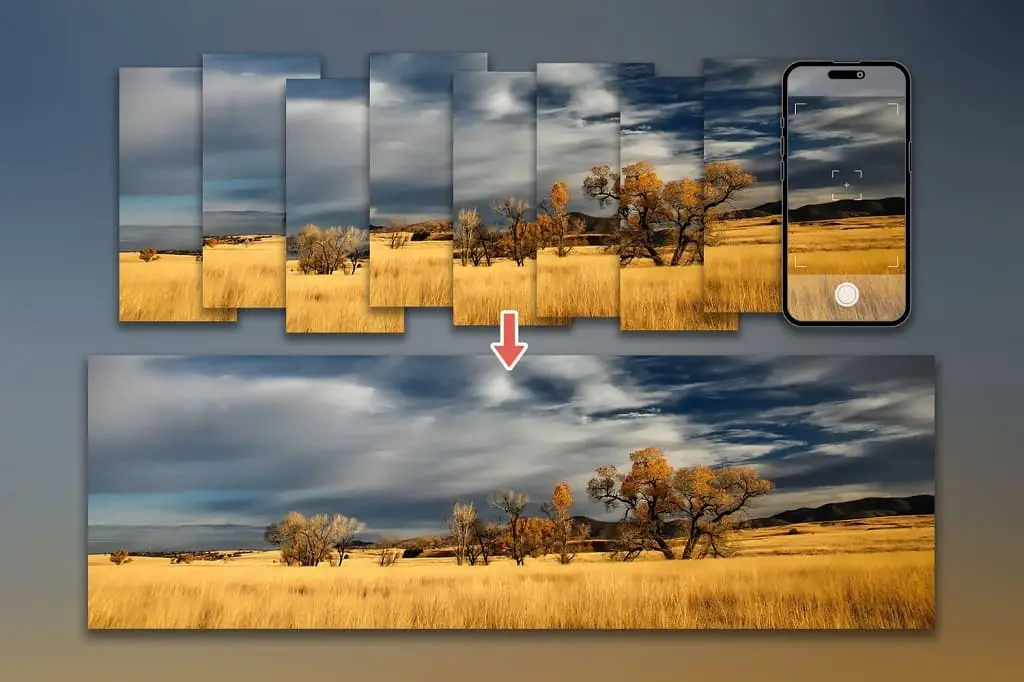
\includegraphics[width=0.92\linewidth]{figuras/panorama_stitching.png}
    \end{column}
    \begin{column}{0.5\textwidth}
      \textbf{Rectificación}
      \begin{itemize}
        \item $4$ esquinas $\to$ rectángulo; $H^{-1}$ endereza (CamScanner).
        \item Rectificar $=$ \alert{restaurar el paralelismo}: manda el punto
              de fuga de vuelta al infinito.
      \end{itemize}
      \centering
      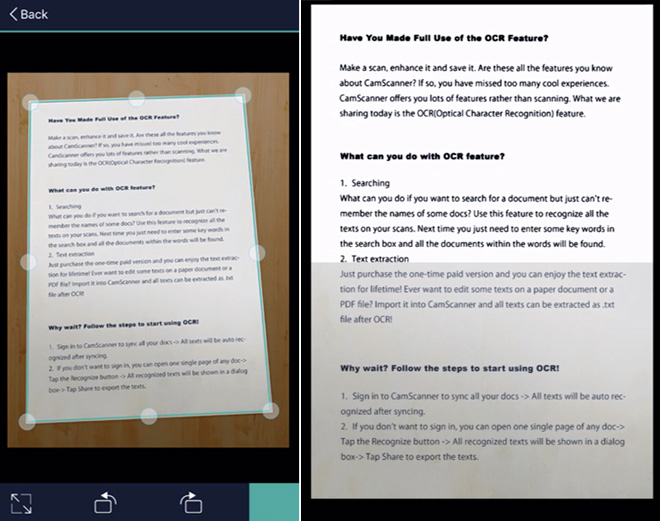
\includegraphics[height=1.9cm]{figuras/escaneo_camscanner.png}\\[2pt]
      \resizebox{0.72\linewidth}{!}{%
      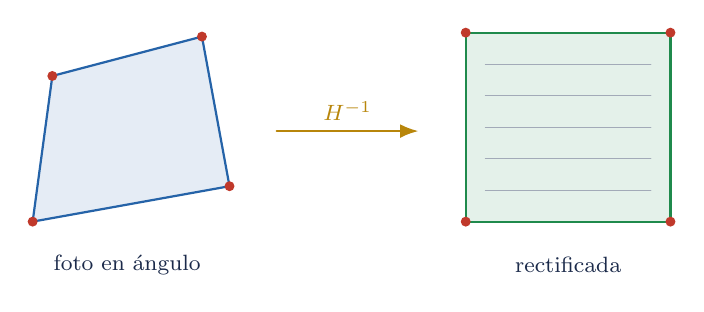
\begin{tikzpicture}[scale=1.0,>=Latex,line cap=round]
        \begin{scope}
          \coordinate (P1) at (0.1,0.0);
          \coordinate (P2) at (2.6,0.45);
          \coordinate (P3) at (2.25,2.35);
          \coordinate (P4) at (0.35,1.85);
          \fill[azul!12] (P1)--(P2)--(P3)--(P4)--cycle;
          \draw[azul,thick] (P1)--(P2)--(P3)--(P4)--cycle;
          \foreach \p in {P1,P2,P3,P4}{ \fill[rojo] (\p) circle (1.8pt); }
          \node[navy,font=\footnotesize] at (1.3,-0.55) {foto en ángulo};
        \end{scope}
        \draw[->,oro,thick] (3.2,1.15) -- (5.0,1.15)
              node[midway,above,font=\footnotesize,oro]{$H^{-1}$};
        \begin{scope}[xshift=5.6cm]
          \coordinate (Q1) at (0,0);
          \coordinate (Q2) at (2.6,0);
          \coordinate (Q3) at (2.6,2.4);
          \coordinate (Q4) at (0,2.4);
          \fill[verde!12] (Q1)--(Q2)--(Q3)--(Q4)--cycle;
          \draw[verde,thick] (Q1)--(Q2)--(Q3)--(Q4)--cycle;
          \foreach \p in {Q1,Q2,Q3,Q4}{ \fill[rojo] (\p) circle (1.8pt); }
          \foreach \y in {0.4,0.8,1.2,1.6,2.0}{
            \draw[gris!70,thin] (0.25,\y) -- (2.35,\y);
          }
          \node[navy,font=\footnotesize] at (1.3,-0.55) {rectificada};
        \end{scope}
      \end{tikzpicture}}
    \end{column}
  \end{columns}
\end{frame}

% ======================================================================
% 21. GRÁFICOS POR GPU: MALLA Y TRASLACIÓN LINEAL
% ======================================================================
\begin{frame}{Gráficos por GPU: malla y traslación lineal}
  \begin{columns}[T]
    \begin{column}{0.5\textwidth}
      \begin{itemize}
        \item Un modelo 3D $=$ \textbf{malla de vértices} en triángulos
              (conejo de Stanford).
        \item En el pipeline:
              \vspace{-4pt}
              \[
                \small\texttt{gl\_Position} = P\cdot M\cdot
                \begin{pmatrix}X\\Y\\Z\\1\end{pmatrix}.
              \]
              \vspace{-12pt}
        \item La \textbf{traslación}, no lineal en $\R^3$, \alert{sí} lo es en
              $\R^4$:
              \vspace{-4pt}
              \[
                \small T(t)=\begin{pmatrix}1&0&0&t_x\\0&1&0&t_y\\0&0&1&t_z\\0&0&0&1\end{pmatrix}.
              \]
              \vspace{-12pt}
        \item Componer transformaciones $=$ \textbf{un solo producto}
              matricial.
      \end{itemize}
    \end{column}
    \begin{column}{0.5\textwidth}
      \centering
      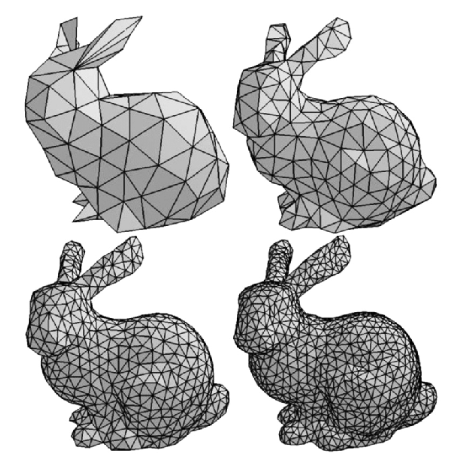
\includegraphics[width=0.72\linewidth]{figuras/malla_conejo.png}
    \end{column}
  \end{columns}
\end{frame}

% ======================================================================
% 22. VISOR LiDAR PROPIO (QR)
% ======================================================================
\begin{frame}{Visor LiDAR propio}
  \begin{columns}[T]
    \begin{column}{0.58\textwidth}
      \begin{itemize}
        \item Nube de puntos \textbf{PandaSet} renderizada con Three.js.
        \item El \emph{mismo} pipeline de GPU: cada punto pasa por
              $P\cdot M$.
        \item Dos cámaras conviven:
              \begin{itemize}
                \item \textbf{virtual} (el usuario orbita la escena);
                \item \textbf{real} $P=K[R\mid t]$ (la del sensor del coche).
              \end{itemize}
      \end{itemize}
      \vspace{0.2cm}
      \begin{block}{Enlaces}
        {\footnotesize
        Demo: \alert{\texttt{https://demo-lidar.cnexans.com}}\\
        Código: \texttt{github.com/cnexans/demo-visualizacion-lidar-webgl}}
      \end{block}
    \end{column}
    \begin{column}{0.42\textwidth}
      \centering
      \qrcode[height=3.4cm]{https://demo-lidar.cnexans.com}\\[4pt]
      {\footnotesize\color{gris} Escaneá para la \textbf{demo en vivo}}
    \end{column}
  \end{columns}
\end{frame}

% ======================================================================
% 23. CONCLUSIÓN + REFLEXIÓN FINAL
% ======================================================================
\begin{frame}{Conclusión}
  \begin{itemize}
    \item \textbf{Coordenadas homogéneas:} un lenguaje uniforme, con el
          infinito \emph{incorporado}; punto y recta en pie de igualdad.
    \item La simetría de $\inc{P}{\ell}=0$ eleva la \textbf{dualidad} a
          teorema: cada resultado trae su dual gratis.
    \item Una sola idea une la \emph{teoría} (Desargues, Pascal/Brianchon) y
          la \emph{práctica} (cámaras, panorámicas, GPU, LiDAR).
  \end{itemize}
  \vspace{0.5cm}
  \begin{block}{}
    \centering\itshape
    «Mirar con cuidado los objetos dentro de una habitación nos permite, a
    veces, entender la naturaleza de la habitación misma.»
  \end{block}
  \vspace{0.3cm}
  \centering{\color{gris}\small ¡Gracias! \quad Carlos Nexans}
\end{frame}

\end{document}
